% VibePrompt — User Manual and NLP Implementation Guide
% Compile: pdflatex VIBEPROMPT_USER_MANUAL.tex  (run twice for TOC)
\documentclass[11pt,a4paper]{article}

\usepackage[margin=2.2cm,headheight=14pt]{geometry}
\usepackage[T1]{fontenc}
\usepackage[utf8]{inputenc}
\usepackage{lmodern}
\usepackage{graphicx}
\usepackage{booktabs}
\usepackage{tabularx}
\usepackage{array}
\usepackage{longtable}
\usepackage{multirow}
\usepackage{enumitem}
\usepackage{xcolor}
\usepackage{hyperref}
\usepackage{fancyhdr}
\usepackage{titlesec}
\usepackage{caption}
\usepackage{float}
\usepackage{setspace}

\hypersetup{
  colorlinks=true,
  linkcolor=black,
  urlcolor=blue!50!black,
  citecolor=black
}

\definecolor{vpmuted}{HTML}{4B5563}
\definecolor{vpactive}{HTML}{2563EB}
\definecolor{vpblock}{HTML}{DC2626}

\newcommand{\placeholder}[1]{\textit{[#1]}}
\newcommand{\appname}{VibePrompt}

\pagestyle{fancy}
\fancyhf{}
\fancyhead[L]{\appname}
\fancyhead[R]{\placeholder{Team name}}
\fancyfoot[L]{User manual / 1.0}
\fancyfoot[R]{\thepage}
\renewcommand{\headrulewidth}{0.4pt}
\renewcommand{\footrulewidth}{0.4pt}

\titleformat{\section}{\large\bfseries}{\thesection}{0.8em}{}
\titleformat{\subsection}{\normalsize\bfseries}{\thesubsection}{0.8em}{}
\titleformat{\subsubsection}{\normalsize\bfseries}{\thesubsubsection}{0.8em}{}

\setlist[itemize]{leftmargin=1.4em, itemsep=0.2em}
\setlist[enumerate]{leftmargin=1.4em, itemsep=0.25em}

\renewcommand{\arraystretch}{1.25}
\newcolumntype{L}[1]{>{\raggedright\arraybackslash}p{#1}}
\newcolumntype{Y}{>{\raggedright\arraybackslash}X}

\begin{document}
\pagenumbering{roman}

%==============================================================================
% TITLE PAGE
%==============================================================================
\begin{titlepage}
  \centering
  {\large \placeholder{Project title} \hfill \placeholder{Team name}\par}
  \vspace{2.5cm}
  {\Large NATURAL LANGUAGE PROCESSING COURSE PROJECT\par}
  \vspace{1.8cm}
  {\Huge\bfseries \appname\par}
  \vspace{0.6cm}
  {\Large User Manual and NLP Implementation Guide\par}
  \vspace{1.2cm}
  {\large
  \appname{} helps developers and technical founders stress-test a product idea
  before they spend coding-agent tokens, using natural-language project
  descriptions and chat.\par}
  \vspace{1.5cm}

  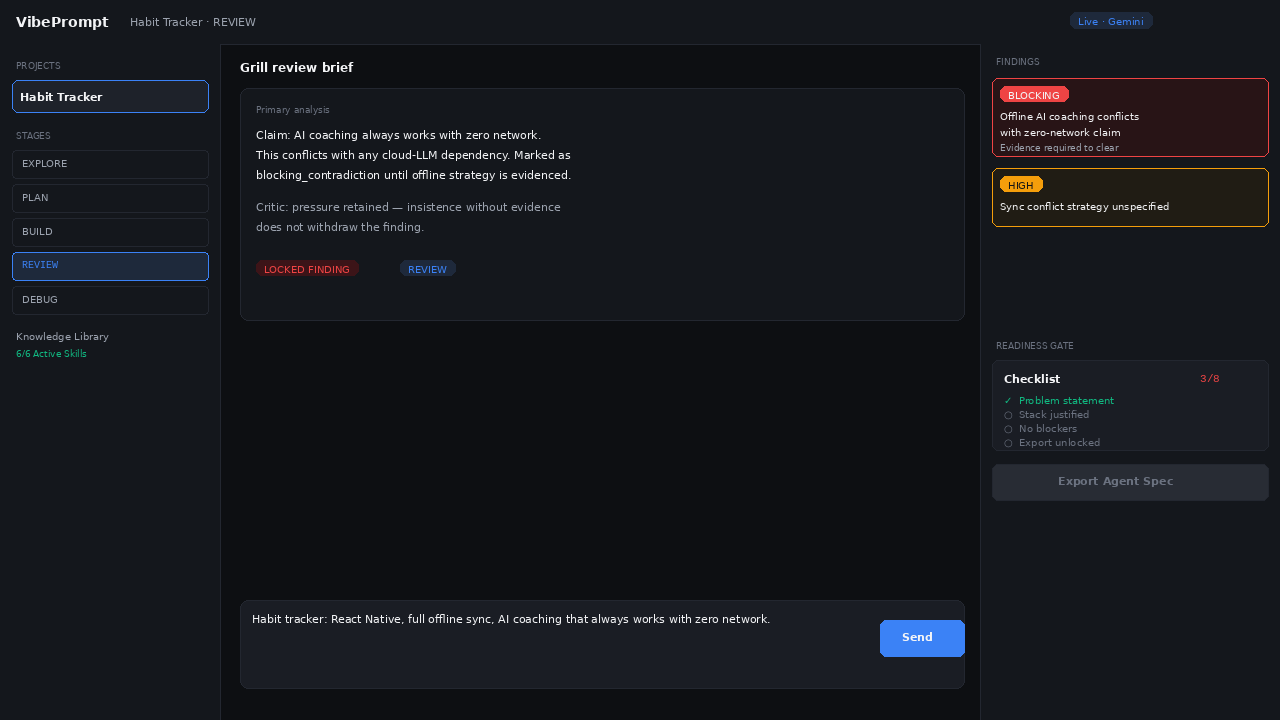
\includegraphics[width=0.92\textwidth]{figures/fig1_workbench_overview.png}
  \captionof{figure}{\appname{} workbench showing a Grill review turn, open findings, and the Readiness Gate.}
  \label{fig:overview}

  \vfill
  {\small Manual version 1.0 · \placeholder{Date}}
\end{titlepage}
\pagenumbering{arabic}
\setcounter{page}{1}

%==============================================================================
% PROJECT AND TEAM
%==============================================================================
\noindent{\large \placeholder{Project title} \hfill \placeholder{Team name}}

\section*{Project and team}
\addcontentsline{toc}{section}{Project and team}

\begin{tabularx}{\textwidth}{@{}L{4.2cm}Y@{}}
\toprule
Team name & \placeholder{Name} \\
Team number & \placeholder{Number, if assigned} \\
\bottomrule
\end{tabularx}

\vspace{0.8em}
\begin{tabularx}{\textwidth}{@{}Y L{3.2cm} Y@{}}
\toprule
\textbf{Team member} & \textbf{Roll number / ID} & \textbf{Project contribution} \\
\midrule
\placeholder{Full name} & \placeholder{ID} & \placeholder{Feature, design, NLP or testing work} \\
\placeholder{Full name} & \placeholder{ID} & \placeholder{Specific contribution} \\
\placeholder{Full name} & \placeholder{ID} & \placeholder{Specific contribution} \\
\bottomrule
\end{tabularx}

\vspace{0.8em}
\begin{tabularx}{\textwidth}{@{}L{4.2cm}Y@{}}
\toprule
Course and section & \placeholder{Course code, course name and section} \\
Department / institution & \placeholder{Department and institution} \\
Faculty guide & \placeholder{Name, if applicable} \\
Manual version and date & 1.0 · \placeholder{Date} \\
\bottomrule
\end{tabularx}

\newpage

%==============================================================================
% PRODUCT OVERVIEW
%==============================================================================
\section*{Product overview}
\addcontentsline{toc}{section}{Product overview}

\subsection*{About the app and contents}
\subsubsection*{What the app does}
Developers and founders often jump into coding agents with vague scope,
contradictory requirements, or unjustified stack choices. \appname{} accepts a
project description and follow-up chat, runs adversarial \textbf{Grill} review
with structured findings, and unlocks \textbf{Export Agent Spec} only after a
deterministic readiness checklist passes. The result is a locked, exportable
project state aimed at fewer wasted agent runs.

\subsubsection*{When to use it}
\begin{tabularx}{\textwidth}{@{}Y Y Y@{}}
\toprule
\textbf{User goal} & \textbf{Feature to use} & \textbf{What the user receives} \\
\midrule
Challenge weak assumptions before building
  & Grill review (REVIEW stage)
  & Open findings with severity, evidence requirements, and resolution notes \\
\addlinespace
Lock a project so coding agents can implement safely
  & Readiness Gate \(\rightarrow\) Export Agent Spec
  & Cursor / Antigravity / Codex agent prompts once \texttt{implementation\_ready} \\
\addlinespace
Shape ideas without premature commitment
  & EXPLORE / PLAN stages (Chat or Brainstorm)
  & Structured project state updates without forcing export \\
\bottomrule
\end{tabularx}

\subsubsection*{Contents}
\tableofcontents

\vspace{0.6em}
\subsubsection*{Who should read which sections}
\begin{itemize}
  \item \textbf{First-time users} --- Start with Getting started, then follow the illustrated walkthrough.
  \item \textbf{Faculty and reviewers} --- Use the worked example to check how each NLP method contributes to the result.
\end{itemize}

\newpage

%==============================================================================
% GETTING STARTED
%==============================================================================
\section{Getting started}
\label{sec:getting-started}

\subsection{What you need}
\begin{tabularx}{\textwidth}{@{}L{3.6cm}Y@{}}
\toprule
\textbf{Requirement} & \textbf{Details for this app} \\
\midrule
Platform and access
  & Modern browser (Chrome, Firefox, Edge, Safari). Local demo: frontend at
    \texttt{http://localhost:5173}, API at \texttt{http://127.0.0.1:8000}.
    Optional Android APK via Capacitor against a hosted HTTPS API. \\
\addlinespace
Permissions or account
  & Guest JWT is minted automatically for short sessions. Sign-in is available
    for registered users, free-tier quota, BYOK keys, and Knowledge Library admin flows. \\
\addlinespace
Supported input
  & English natural-language project descriptions and chat turns. Optional BYOK
    API keys (Gemini / OpenRouter / Groq / Qwen). Without provider keys the app
    runs \textbf{offline heuristic mode} (demo/tests only --- not live adversarial review). \\
\bottomrule
\end{tabularx}

\subsection{Open the app for the first time}
\begin{enumerate}
  \item Start the backend with
        \texttt{uvicorn\ app.main:app\ --reload\ --port\ 8000}
        from \texttt{backend/}, and the frontend with \texttt{npm\ run\ dev}
        from \texttt{frontend/}, or open the deployed SPA URL your team provides.
  \item On first load the SPA bootstraps a guest session (\texttt{POST /api/auth/guest}).
        Sign in if you need free-tier generations, BYOK, or Knowledge Library.
  \item You land on the workbench: left rail (projects and stages), center composer,
        right inspector (Readiness Gate and findings). Create or select a project to begin.
\end{enumerate}

\begin{figure}[H]
  \centering
  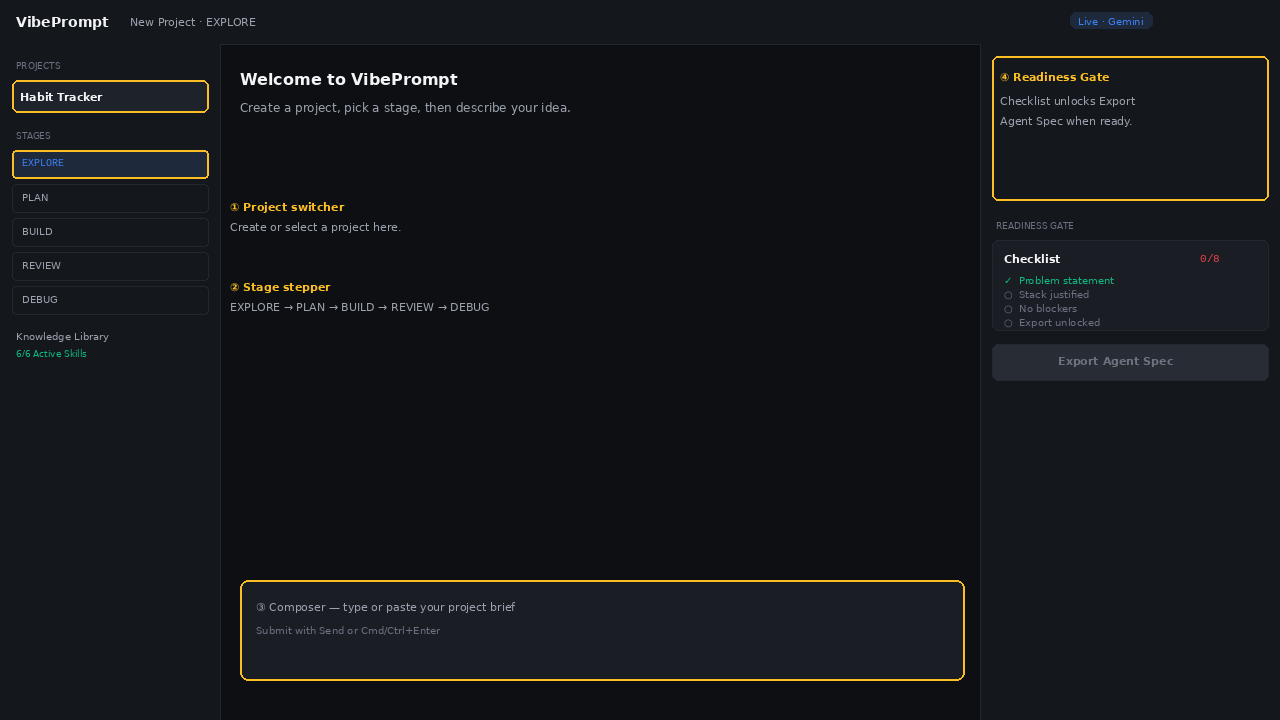
\includegraphics[width=\textwidth]{figures/fig2_workbench_home.png}
  \caption{Workbench home. Annotated: project switcher, stage stepper
  (EXPLORE \(\rightarrow\) PLAN \(\rightarrow\) BUILD \(\rightarrow\) REVIEW \(\rightarrow\) DEBUG),
  composer, and Readiness Gate panel.}
  \label{fig:home}
\end{figure}

\subsection{Find your way around}
\begin{tabularx}{\textwidth}{@{}L{3.4cm}Y@{}}
\toprule
\textbf{Control} & \textbf{Where it is and what it opens} \\
\midrule
Left rail & Project switcher, behavioural stage stepper, Knowledge Library status (\texttt{N/N Active Skills}) \\
Center workspace & Conversation / review briefs; type or paste project text; submit with Send or Cmd/Ctrl+Enter \\
Right inspector & Readiness Gate score/checklist, open findings (including blocking contradictions), Export Agent Spec CTA \\
Top bar & Breadcrumb, inference mode pill, theme and export shortcuts \\
\bottomrule
\end{tabularx}

\newpage

%==============================================================================
% HOW TO USE
%==============================================================================
\section{How to use the app}
\label{sec:how-to-use}

Task: describe a small product idea, run Grill review, resolve blockers, then
export an agent-ready spec. Use one example throughout the three steps.

\subsection{Enter the input}
Open or create a project. In the composer, paste a short project brief --- for example:
\begin{quote}
\textit{``Build a habit tracker with React Native, offline sync, and AI coaching
that always works without a network.''}
\end{quote}

\begin{figure}[H]
  \centering
  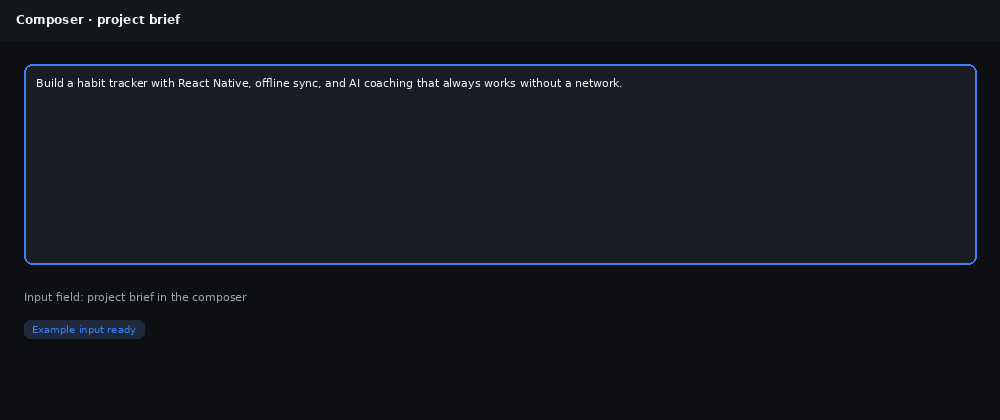
\includegraphics[width=0.95\textwidth]{figures/fig3a_composer_input.png}
  \caption{Input field containing the example project brief.}
  \label{fig:input}
\end{figure}

\subsection{Run the feature}
Select \textbf{REVIEW} (or let intent routing choose Grill review). Send the message.
The backend runs primary analysis (and an optional critic on review turns),
validates the reply, and updates structured project state.

\begin{figure}[H]
  \centering
  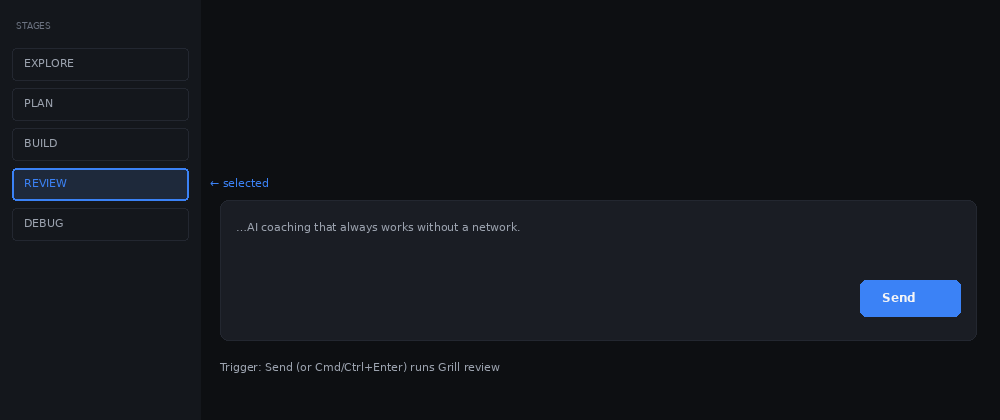
\includegraphics[width=0.95\textwidth]{figures/fig3b_review_send.png}
  \caption{REVIEW stage selected and Send trigger.}
  \label{fig:run}
\end{figure}

\subsection{Read the result}
In the center pane, read the Grill brief. In the right inspector, open findings
list severity and evidence requirements. Resolve findings with counterevidence
(a \texttt{blocking\_contradiction} cannot be dismissed without state/artifact support).
When the Readiness Gate shows ready, use \textbf{Export Agent Spec} and choose
Cursor, Antigravity, or Codex.

\begin{figure}[H]
  \centering
  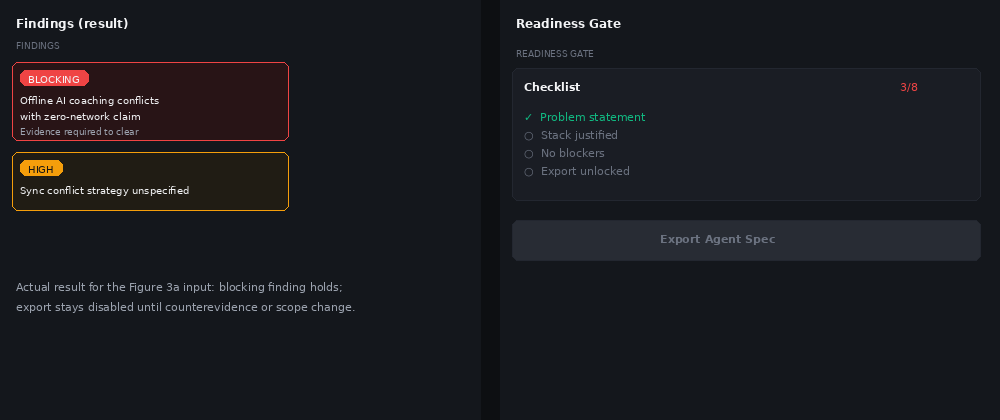
\includegraphics[width=0.95\textwidth]{figures/fig3c_findings_readiness.png}
  \caption{Actual result for the input shown in Figure~\ref{fig:input}: blocking finding and incomplete readiness.}
  \label{fig:result}
\end{figure}

\newpage

%==============================================================================
% FEATURES
%==============================================================================
\section{Features and a worked example}
\label{sec:features}

\subsection{Feature details}
{\small
\begin{tabularx}{\textwidth}{@{}L{2.6cm} L{2.8cm} L{3.0cm} Y@{}}
\toprule
\textbf{Feature} & \textbf{When to use it} & \textbf{How to open it} & \textbf{Output to expect} \\
\midrule
Grill review
  & Challenge unsupported claims, contradictions, and weak stack choices
  & Stage \(\rightarrow\) REVIEW (or grill intent in chat)
  & Structured findings with severity; optional critic pass; updated project state \\
\addlinespace
Readiness Gate
  & Decide whether the project is safe to hand to a coding agent
  & Right inspector --- Readiness checklist
  & Pass/fail checklist; unlocks export when \texttt{implementation\_ready} \\
\addlinespace
Export Agent Spec
  & Produce Cursor / Antigravity / Codex prompts
  & Export Agent Spec CTA (enabled after readiness)
  & Agent-ready Markdown / prompt payloads \\
\addlinespace
Knowledge Library / Active Skills
  & Inject approved book-derived principles into chat
  & Left rail \(\rightarrow\) Knowledge Library (admin for uploads)
  & Ranked short principle block --- not full book text \\
\addlinespace
BYOK / free tier
  & Continue live LLM review after free quota
  & Settings / API key modal on \texttt{429}
  & Encrypted user keys; provider status in replies \\
\bottomrule
\end{tabularx}
}

\subsection{Worked example for Grill review}
\textbf{Purpose.} Show how an overstated offline + AI claim becomes a finding
the user must resolve before export.

\begin{tabularx}{\textwidth}{@{}L{3.4cm}Y@{}}
\toprule
\textbf{Record} & \textbf{From one actual run} \\
\midrule
Input
  & ``Habit tracker: React Native, full offline sync, AI coaching that always works with zero network.'' \\
\addlinespace
Settings
  & Stage = REVIEW; live providers configured (or note offline heuristic banner if demoing without keys) \\
\addlinespace
Output
  & Finding such as a \texttt{blocking\_contradiction}: always-on AI coaching conflicts with zero-network requirement; readiness remains incomplete until resolved \\
\addlinespace
Interpretation
  & The contradiction is tied to the ``always works without network'' + ``AI coaching'' pair. Narrow the claim (e.g.\ on-device model, degraded offline mode) or drop one requirement, then re-run review \\
\bottomrule
\end{tabularx}

\subsection{A case that needs review}
\begin{itemize}
  \item \textbf{Input variation:} Change ``always works without a network'' to
        ``queues coaching requests until online.''
  \item \textbf{What happened:} The hard offline/AI contradiction should soften or clear;
        remaining findings may cover sync conflict resolution or stack justification.
        Still verify stack and sync claims manually before treating readiness as final.
\end{itemize}

\newpage

%==============================================================================
% NLP IMPLEMENTATION
%==============================================================================
\section{How NLP is implemented}
\label{sec:nlp}

\appname{} performs intent-aware dialogue understanding, structured information
extraction into project state, adversarial claim critique, and (on review)
optional multi-model critic reconciliation. The user-facing Grill review,
findings lifecycle, and readiness-gated export all depend on this pipeline.

\subsection{Map course concepts to the app}
{\footnotesize
\begin{tabularx}{\textwidth}{@{}L{2.4cm} L{2.6cm} Y L{2.6cm}@{}}
\toprule
\textbf{App feature} & \textbf{NLP concept} & \textbf{Actual method or component} & \textbf{Visible effect} \\
\midrule
Mode routing (EXPLORE--DEBUG)
  & Intent classification / dialogue act selection
  & Cue regexes + sticky follow-ups in \texttt{app/grill/modes.py}; explicit UI mode wins
  & Stage badge and reply behaviour \\
\addlinespace
Grill findings
  & Information extraction + claim verification
  & LLM primary analysis \(\rightarrow\) \texttt{state\_patch} \(\rightarrow\) \texttt{apply\_state\_patch}; contradiction detection
  & Open findings with severity and evidence requirements \\
\addlinespace
Critic pass (REVIEW)
  & Multi-agent / dual-model critique
  & Primary provider chain + Groq critic when \texttt{CRITIC\_ENABLED}
  & Stronger review briefs; critic does not rewrite conversational replies \\
\addlinespace
Readiness + export
  & Deterministic compilation / constrained NLG
  & \texttt{app/compilation} readiness gate + Markdown / agent-prompt compilers
  & Export enabled only when checklist passes \\
\addlinespace
Knowledge / skills
  & Retrieval-augmented generation (RAG-lite)
  & Book-to-Skill abstracts \(\rightarrow\) ranked principle injection
  & Short principle block in Chat / Brainstorm / Grill \\
\bottomrule
\end{tabularx}
}

\subsection{Explain one feature in detail: Grill review}
\paragraph{Input preparation.}
The engine builds a mode-scoped context snapshot (not a full history dump):
problem statement, decisions, stack, open findings, and recent messages.
Skills inject a short ranked principle block when approved skills are active.
Trivial greetings may skip model debate for cost control.

\paragraph{Processing.}
One user turn flows through: mode resolve \(\rightarrow\) policy \(\rightarrow\)
context retrieval \(\rightarrow\) primary LLM (Gemini \(\rightarrow\) OpenRouter \(\rightarrow\)
Groq failover, or offline heuristics) \(\rightarrow\) optional critic on REVIEW \(\rightarrow\)
validation \(\rightarrow\) state apply (dedupe, contradiction surfacing) \(\rightarrow\) persist.
Findings such as \texttt{blocking\_contradiction} require counterevidence in
state/artifacts; insistence without evidence does not withdraw them.

\paragraph{Output in the interface.}
The assistant brief appears in the center workspace. Findings and readiness
update in the right inspector --- the same surfaces shown in
Figure~\ref{fig:result} and the worked example in Section~\ref{sec:features}.

\subsection{What the team built}
\begin{itemize}
  \item \textbf{Team implementation:} Grill orchestration, finding lifecycle and readiness gate,
        project-state persistence, React workbench UI, export compilers, guest JWT / BYOK /
        free-tier routing, Knowledge Library Book-to-Skill pipeline.
  \item \textbf{Reused components:} External LLM APIs (Gemini, OpenRouter, Groq,
        optional Qwen); FastAPI; React + TypeScript + Vite; SQLite (local) /
        PostgreSQL (prod). Model IDs are configurable via environment variables.
\end{itemize}

\newpage

%==============================================================================
% WORKFLOW DIAGRAM
%==============================================================================
\section{NLP workflow diagram}
\label{sec:workflow}

Use this page to show how one user action becomes one visible result.
Figure~\ref{fig:workflow} labels what passes from one component to the next.

\begin{figure}[H]
  \centering
  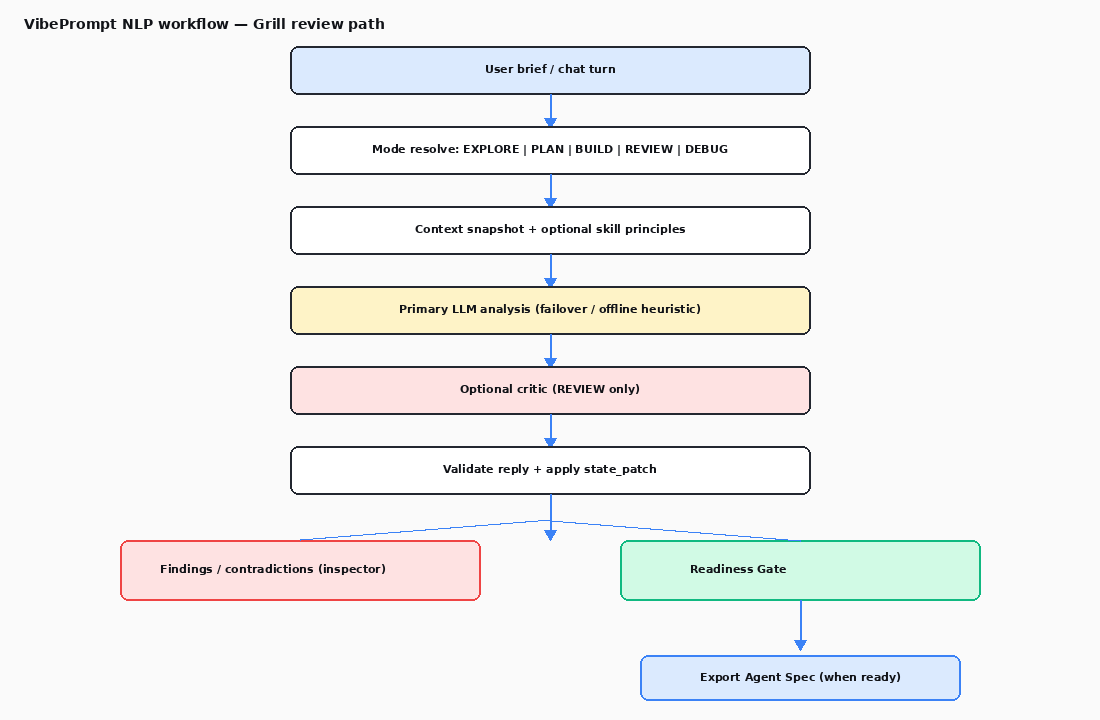
\includegraphics[width=0.92\textwidth]{figures/fig4_nlp_workflow.png}
  \caption{Grill review processing a project chat turn and returning findings plus updated readiness.}
  \label{fig:workflow}
\end{figure}

\subsection{Trace one input through the diagram}
\begin{tabularx}{\textwidth}{@{}L{3.6cm}Y@{}}
\toprule
\textbf{Point in the flow} & \textbf{What to put here} \\
\midrule
Input
  & Habit-tracker brief claiming full offline AI coaching \\
\addlinespace
Intermediate stage
  & Mode = REVIEW; context includes prior stack/decisions; primary model returns analysis + \texttt{state\_patch}; critic may add pressure on the offline/AI claim \\
\addlinespace
Final output
  & Finding listed in the inspector; readiness incomplete; user sees recovery path via evidence or scope change; export stays disabled until gate passes \\
\bottomrule
\end{tabularx}

\newpage

%==============================================================================
% TROUBLESHOOTING
%==============================================================================
\section{Troubleshooting and reference}
\label{sec:help}

\subsection{Troubleshooting}
{\small
\begin{tabularx}{\textwidth}{@{}Y Y Y@{}}
\toprule
\textbf{What the user sees} & \textbf{What to check} & \textbf{What to do next} \\
\midrule
Banner: ``Offline heuristic mode --- not live adversarial review''
  & No provider keys, or \texttt{DEMO\_MODE=true}
  & Add \texttt{GEMINI\_API\_KEY} / \texttt{OPENROUTER\_API\_KEY} / \texttt{GROQ\_API\_KEY} (or BYOK), restart API, confirm health endpoint \\
\addlinespace
\texttt{429} / API key modal
  & Free-tier generations exhausted or rate limit
  & Configure BYOK in the modal; wait if rate-limited \\
\addlinespace
Export Agent Spec disabled
  & Open findings or failed readiness checklist
  & Resolve blockers with evidence; re-run REVIEW; confirm \texttt{implementation\_ready} \\
\addlinespace
Guest session ends / access error
  & Expired guest JWT
  & Refresh the page to mint a new guest token, or sign in \\
\addlinespace
Android APK cannot reach API
  & \texttt{VITE\_API\_BASE\_URL} and \texttt{CORS\_ORIGINS}
  & Point APK at HTTPS API; add Capacitor WebView origin to API CORS \\
\bottomrule
\end{tabularx}
}

\subsection{Limits and responsible use}
\begin{itemize}
  \item \textbf{Known limitation:} Offline heuristics and weak or contradictory user text can
        produce incomplete findings. Treat Grill output as advisory; verify stack and compliance
        claims yourself before shipping.
  \item \textbf{Handling user input:} Project text and chat are sent to the configured LLM providers
        (platform keys or BYOK). Retention follows those providers' policies --- do not submit
        secrets, credentials, or personal data you are not allowed to share. BYOK keys are stored
        encrypted; raw keys are never returned by the API. Knowledge uploads must be rights-confirmed;
        pirate sources are refused.
\end{itemize}

\subsection{Glossary and references}
\begin{tabularx}{\textwidth}{@{}L{4.2cm}Y@{}}
\toprule
\textbf{Term} & \textbf{Meaning} \\
\midrule
Readiness Gate & Deterministic checklist/score that unlocks agent export \\
Finding & Challenged claim with severity and evidence requirements \\
Blocking contradiction & Finding kind that requires state/artifact counterevidence to clear \\
Grill review & Adversarial REVIEW-mode analysis of the project \\
BYOK & Bring your own API key for live inference after free quota \\
Stages & EXPLORE, PLAN, BUILD, REVIEW, DEBUG \\
Export Agent Spec & Primary CTA once readiness passes (Cursor / Antigravity / Codex) \\
Critic & Optional second-model review pass used only in REVIEW \\
\bottomrule
\end{tabularx}

\vspace{0.6em}
\noindent\textbf{References}
\begin{itemize}
  \item Project README --- repository root \texttt{README.md}
  \item Grill mentor architecture --- \texttt{docs/GRILL\_MENTOR\_ARCHITECTURE.md}
  \item Book-to-Skill architecture --- \texttt{docs/BOOK\_TO\_SKILL\_ARCHITECTURE.md}
  \item Deployment and recovery --- \texttt{docs/DEPLOYMENT\_AND\_RECOVERY.md}
  \item Provider / model cards --- Gemini, OpenRouter, Groq, Qwen documentation for the configured model IDs
\end{itemize}

\subsection{Support and version history}
\textbf{Support:} \placeholder{Team contact or course-approved channel}.
When reporting an issue, include feature name, a non-sensitive example input,
and the observed result (plus whether the offline heuristic banner was shown).

\vspace{0.6em}
\begin{tabularx}{\textwidth}{@{}L{3cm} L{3cm} Y@{}}
\toprule
\textbf{Manual version} & \textbf{Date} & \textbf{Change} \\
\midrule
1.0 & \placeholder{Date} & Initial \appname{} draft from NLP course template \\
\bottomrule
\end{tabularx}

\vspace{1.2em}
{\small\color{vpmuted}
\noindent\textit{Note on figures.} Figures~\ref{fig:overview}--\ref{fig:result} are design-faithful
UI mockups of the \appname{} workbench for print. Replace them with live screenshots from your
demonstration before final submission if the course requires captured UI.}

\end{document}
